\section{Modélisation}

\subsection{Diagramme des cas d’utilisations}


\subsection{Diagramme de classes C\#}

Sur le diagramme, une classe UI_Menu est présente. Elle représente les classes d'interface que nous utiliserons pour afficher des menus d'informations à l'utilisateur.
Nous utiliserons de préférence les classes rajoutées par la dernière version de MiddleVR (1.6.0), car ardaptées à la 3D et à la réalité virtuelle.
Cette version étant disponible seulement depuis la semaine précédente, nous n'avons pas eu l'occasion d'étudier l'architecture proposée pour cette partie.
Dans le cas où nous ne pourrions intégrer ces fonctionnalités, nous utiliserons une manière plus basique pour l'affichage, telle que des textures appliqués sur des plans.
\newline
La classe \textit{RemoteCommand} permet d'afficher la télécommande qui contrôle les équipements domotiques. 
Elle utilisera si possible les classes d'interface MiddleVR, et permettra d'interragir avec l'appartement.

\begin{figure}[p]
    \centering
    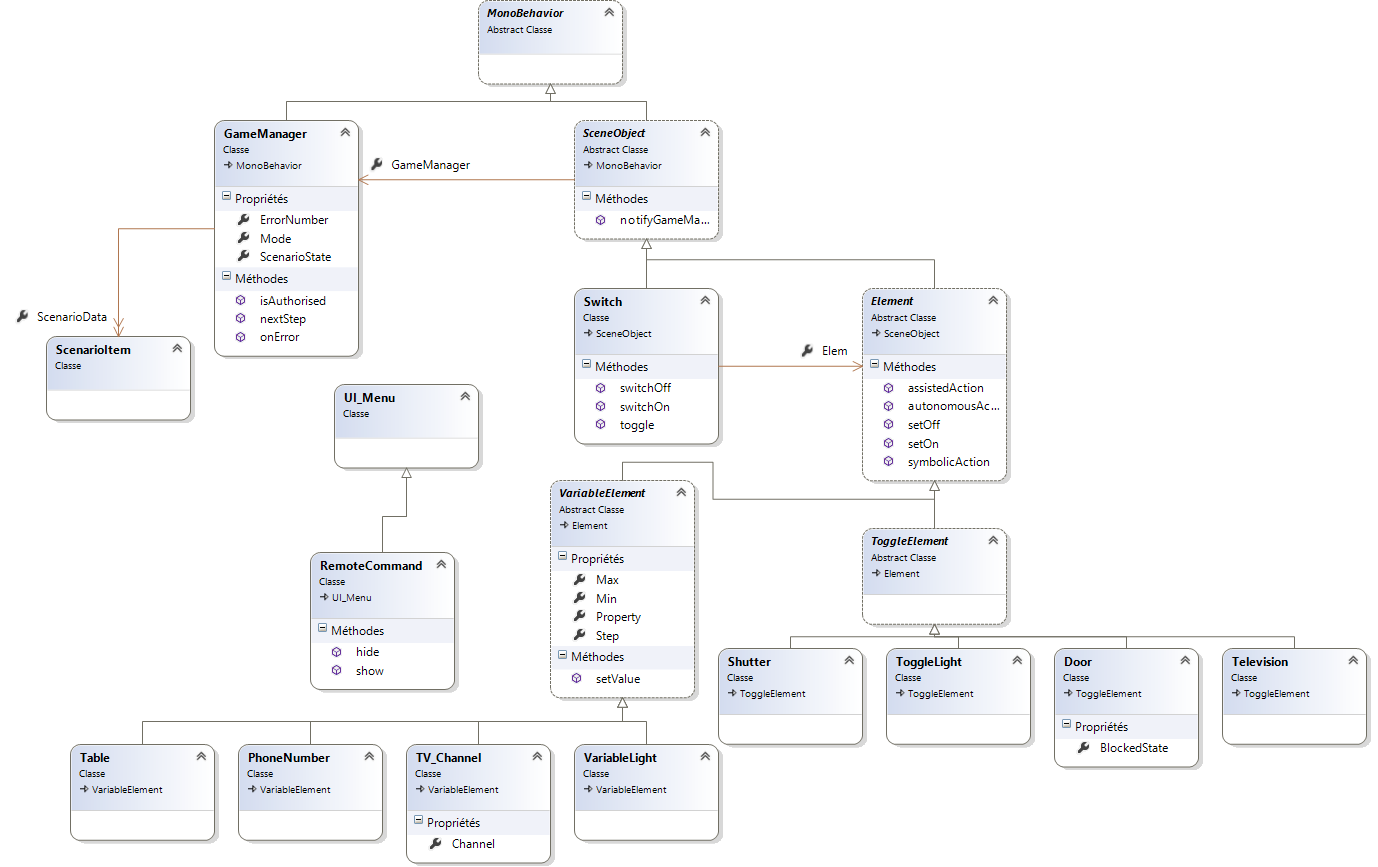
\includegraphics[width=0.8\textwidth]{img/diagClasses.png}
    \caption{Diagramme de classes}
    \label{fig:class_diagram}
\end{figure}
 
On distingue deux types d'éléments sur lesquels ont peut interragir : Ceux avec un état allumé/éteins, et ceux avec un état variable, comme la table et sa hauteur.
Tout les cas simples seront gérés par des ToggleElement. Les différences entre chaques sous classes se résument à des détails de l'objets.
Une lumière allumé ou éteinte n'est pas géré de la même manière que la hauteur d'un volet.
La classe VariableElement permet de gérer les GameObjects avec une valeur interne; il est possible de d'augmenter les variables de manière incrémentale ou de fixer une valeur directement.
Cette classe inclu une valeur minimale et maximale pour la valeur contrainte, ainsi qu'un pas de déplacement.
Ce pas permet de régler le changement de valeur à chaque clic; par exemple, on choisira 1cm dans le cas de la table, pour que le déplacement soit cohérent avec la réalité.

Ce modèle inclu aussi les spécificités relatives au différents éléments, comme la propriété \textit{BlockedState} des portes qui permet de savoir où le mouvement de la porte à été stoppé la dernière fois, pour ralentir lors du prochain essai.

Toutes ces classes, comme \textit{VariableLight}, \textit{Shutter} ou \textit{Table},  ne disposent pas de variable modélisant leur état courant. 
Il faut prendre en compte que ce sont des scripts associé un objet 3D. 
La valeur actuelle (de hauteur dans le cas de la table par exemple) correspond à une ou plusieurs caractéristiques graphiques de l'objet.
\newline
Pour toutes les informations et les fonctionnalités non liées à un objet en particulier (souvent encapsulé dans un singleton dans un contexte objet), les developpeurs unity préconisent d'associer des scripts à un GameObject n'ayant pas d'éléments graphiques et ne contenant pas d'autres GameObject.
L'accès à ces éléments se fait via le nom du GameObject les contenant, ou via des tags référençant l'élément. Ce GameObject doit être unique ce qui fait que la classe GameManager s'apparente dans l'utilisation à un singleton (bien que n'en étant pas un). 
